\documentclass[../analysisII_notes.tex]{subfiles}
\begin{document}
\section{Aula 20 - 28 de Maio, 2025}
\subsection{Motivações}
\begin{itemize}
	\item Séries de Potências.
\end{itemize}
\subsection{Séries de Potências - Parte I.}
Começamos a partir de algumas propriedades do lim sup e do lim inf.
\begin{prop*}[Propriedades do limsup e do liminf]
	Dada uma sequência numérica \(\{x_{n}\}_{n}\) de números reais, valem:
	\begin{itemize}
		\item[I)] O liminf é sempre menor ou igual que o lim sup, com a igualdade acontecendo apenas se a sequência convergir:
		      \[
			      \liminf_{n\to \infty}x_{n}\leq \limsup_{n\to \infty}x_{n}\;\&\; \liminf_{n\to \infty}x_{n}=\limsup_{n\to \infty}x_{n}=\alpha \Longleftrightarrow x_{n}\overbracket[0pt]{\longrightarrow}^{n\to \infty}\alpha .
		      \]
		\item[II)] A sequência \(\{x_{n}\}_{n}\) é ilimitada inferiormente se, e somente se, \(\liminf_{n\to \infty}x_{n} = -\infty\). Analogamente, a sequência \(\{x_{n}\}_{n}\) é ilimitada superiormente se, e somente se, \(\limsup_{n\to \infty}x_{n} = \infty\);
		\item[III)] Se \(c \geq 0\), então
		      \[
			      \liminf_{n\to \infty}(cx_{n}) = c \liminf_{n\to \infty}x_{n} \quad\&\quad \limsup_{n\to \infty}(cx_{n}) = c \limsup_{n\to \infty}x_{n};
		      \]
		\item[IV)] Se \(\{y_{n}\}_{n}\) é uma sequência que converge até \(\beta > 0\), então
		      \[
			      \limsup_{n\to \infty}(y_{n}x_{n}) = \beta \limsup_{n\to \infty}x_{n} \quad\&\quad \liminf_{n\to \infty}(y_{n}x_{n}) = \beta \liminf_{n\to \infty}x_{n}.
		      \]
	\end{itemize}
\end{prop*}
\hypertarget{root_test}{
	\begin{theorem*}[Teste da Raiz]
		Se \(\sum\limits_{}^{}c_{n}\) for uma série numérica de números reais ou complexos e
		\[
			L\coloneqq \limsup_{n\to \infty}|c_{n}|^{\frac{1}{n}} = \limsup_{n\to \infty}\sqrt[n]{|c_{n}|}\in [0, \infty],
		\]
		temos os seguintes casos:
		\begin{itemize}
			\item[1)] Se \(L < 1\), então a série converge absolutamente;
			\item[2)] Se \(L > 1\), então a série diverge;
			\item[3)] Se \(L = 1\), então o teste é inconclusivo.
		\end{itemize}
	\end{theorem*}
}
Vale lembrar que o teste da raiz ``é mais robusto'' que o teste da razão - existem séries que divergem pelo teste da razão (ou são inconclusivas), mas convergem pelo teste da raiz; porém, toda série que diverge pelo teste da raiz também diverge pelo da razão.
\begin{theorem*}
	Se \(\sum\limits_{}^{}c_{n}\) é uma série numérica com todos os termos não nulos, então
	\[
		\liminf_{n\to \infty}\frac{|c_{n+1}|}{|c_{n}|}\leq \liminf_{n\to \infty}|c_{n}|^{\frac{1}{n}} \leq \limsup_{n\to \infty}|c_{n}|^{\frac{1}{n}}\leq \limsup_{n\to \infty}\frac{|c_{n+1}|}{|c_{n}|}.
	\]
\end{theorem*}
\begin{def*}
	Dada uma sequência \(\{a_{n}\}_{n}\) de números reais ou complexos e um ponto \(x_{0}\) em \(\mathbb{R}\) ou \(\mathbb{C}\), a série de funções
	\[
		f(x) = \sum\limits_{n=0}^{\infty}a_{n}(x-x_{0})^{n}
	\]
	é chamada \textbf{série de potência com coeficientes }\(a_{n}\) \textbf{e centro }\(x_{0}.\quad \square\)
\end{def*}
O problema que iremos explorar é: dada uma série de potências qualquer, queremos determinar o conjunto de pontos para os quais ela converge e criar uma função a partir disso, ou seja, encontrar
\[
	I = \{x\in \mathbb{R}:\; \sum\limits_{}^{}a_{n}(x-x_{0})^{n}\text{ converge}\},
\]
determinar uma função
\begin{align*}
	f: & I\rightarrow \mathbb{R}                                             \\
	   & x\mapsto f(x)\coloneqq \sum\limits_{n=0}^{\infty}a_{n}(x-x_{0})^{n}
\end{align*}
e explorar suas propriedades.
\hypertarget{convergence_radius}{\begin{theorem*}[Raio de Convergência]
		Dada a série de potências \(\sum\limits_{}^{}a_{n}(x-x_{0})^{n}\), considere um número R entre 0 e \(\infty\) dado por
		\[
			\frac{1}{R} \coloneqq \limsup_{n\to \infty}|a_{n}|^{\frac{1}{n}}.
		\]
		\begin{figure}[H]
			\begin{center}
				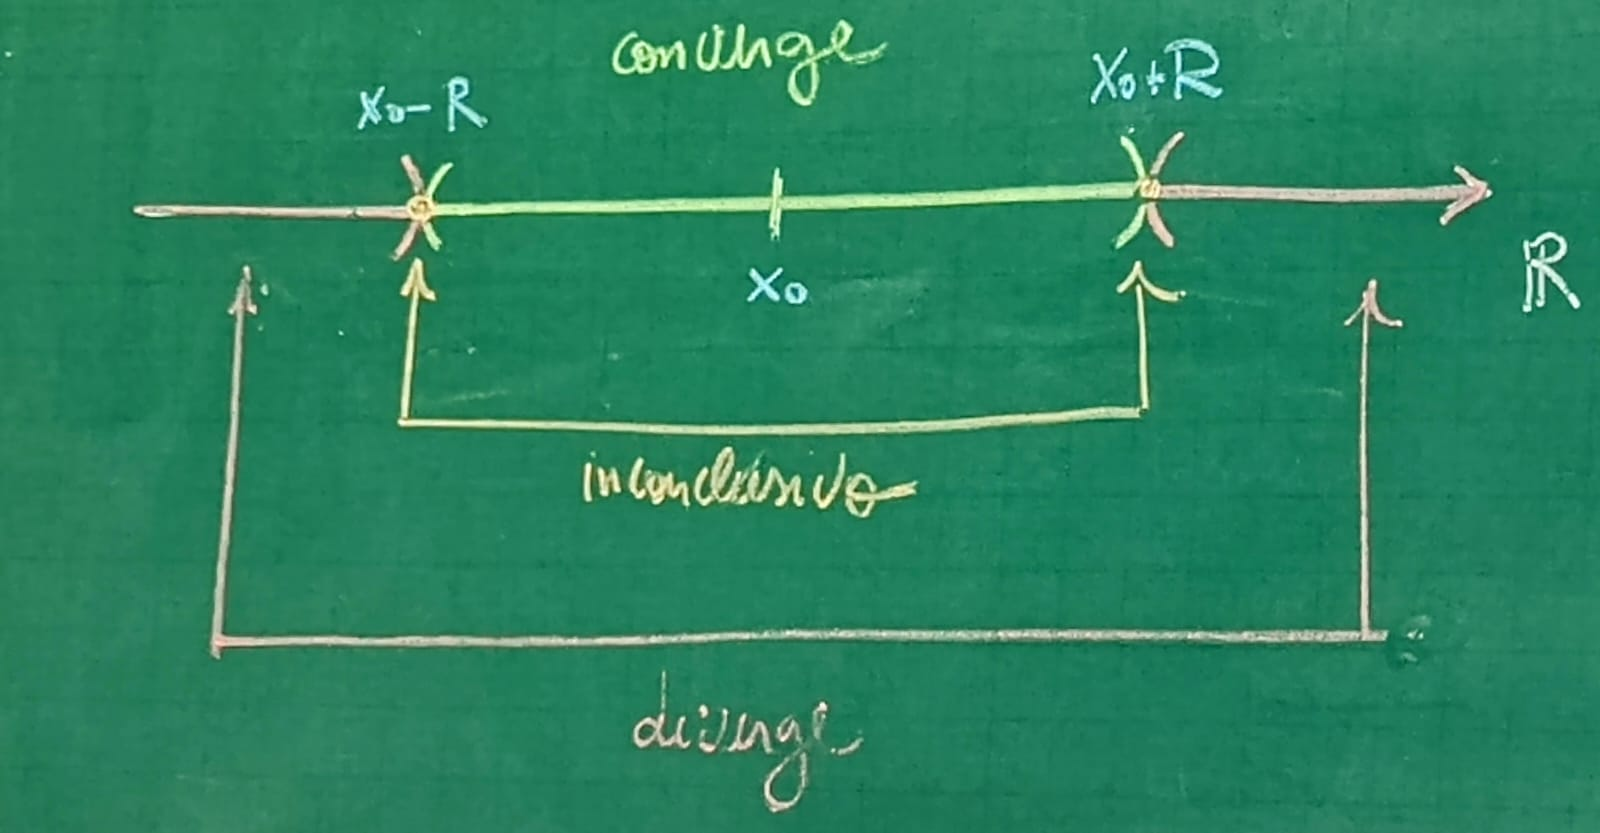
\includegraphics[height=0.4\textheight, width=0.4\textwidth, keepaspectratio]{./Images/convergence_radius_20.png}
			\end{center}
			\caption{com esta definição de R, forma-se um intervalo com extremos \(x_{0}-R\) e \(x_{0} + R\) em torno de x. Chamamos ele de semáforo!}
			\label{convradi20}
		\end{figure}
		Então,
		\begin{itemize}
			\item[i)] Se \(R > 0\), com a possibilidade de ser infinito, e \(|x-x_{0}| < R\), então a série de potências converge absolutamente. Além disso, dado um número positivo menor que R (\(0 < r < R\)), a série de potências, como série de funções, converge uniformemente para qualquer x no intervalo \([x_{0}-r, x_{0}+r]\). Note que se \(R = \infty\), a série converge para todo número real x; por outro lado, se \(R = 0\), então a série de potências só converge quando \(x=x_{0}\);
			\item[ii)] Se \(|x-x_{0}| > R\), então \(\sum\limits_{}^{}a_{n}(x-x_{0})^{n}\) diverge;
			\item[iii)] Se \(|x-x_{0}|=R\), o teorema não tem conclusão.
		\end{itemize}
	\end{theorem*}}
\begin{tcolorbox}[
		skin=enhanced,
		title=Observação,
		fonttitle=\bfseries,
		colframe=black,
		colbacktitle=cyan!75!white,
		colback=cyan!15,
		colbacklower=black,
		coltitle=black,
		drop fuzzy shadow,
		%drop large lifted shadow
	]
	No teorema acima, \(R = 0\) apenas quando \(\limsup_{n\to \infty}|a_{n}|^{\frac{1}{n}} = \infty\); por outro lado, \(R = \infty\) apenas se \(\limsup_{n\to \infty}|a_{n}|^{\frac{1}{n}} = 0.\)
\end{tcolorbox}
\begin{proof*}
	Suponha que \(x_{0} = 0\), sem perda de generalidade, e considere, para x número real qualquer, o valor \(c_{n}\coloneqq a_{n}x^{n}\). Apliquemos o \hyperlink{root_test}{\textit{teste da raiz}} na série dos \(c_{n}\)'s, ou seja, calculemos
	\begin{align*}
		L\coloneqq \limsup_{n\to \infty}|c_{n}|^{\frac{1}{n}} & = \limsup_{n\to \infty}|a_{n}x^{n}|                              \\
		                                                      & = \limsup_{n\to \infty}\biggl[|a_{n}|^{\frac{1}{n}}||x|\biggr]   \\
		                                                      & = |x|\limsup_{n\to \infty}|a_{n}|^{\frac{1}{n}} = \frac{|x|}{R}.
	\end{align*}
	Daí,
	\[
		|x|<R \Rightarrow \frac{|x|}{R} = L < 1,
	\]
	implicando na convergência absoluta da série. Por outro lado,
	\[
		|x|>R \Rightarrow L = \frac{|x|}{R} > 1,
	\]
	concluindo que a série diverge. Finalizando os casos,
	\[
		|x| = R \Rightarrow \frac{|x|}{R} = L = 1,
	\]
	levando à falta de resposta.

	Finalmente, dado r um número tal que \(0 < r < R\) e \(|x| \leq r\), então
	\[
		|a_{n}x|^{n} \leq |a_{n}|r^{n}\eqqcolon M_{n}.
	\]
	Portanto, pelo \hyperlink{weierstrass_m}{\textit{Teste M de Weierstrass}}, a conclusão é a convergência absoluta. \qedsymbol
\end{proof*}
\begin{def*}
	O R obtido no \hyperlink{convergence_radius}{\textit{teorema}} é chamado \textbf{raio de convergência}, e o conjunto
	\[
		I = \{x\in \mathbb{R}:\; \sum\limits_{}^{}a_{n}(x-x_{0})^{n}\text{ converge}\}
	\]
	é chamado \textbf{intervalo de convergência da série.} \(\square\)
\end{def*}
\begin{example}
	Dada a série de potências com centro em 0 e coeficientes todos iguais a 1, ou seja,
	\[
		\sum\limits_{n=0}^{\infty}x^{n},
	\]
	então
	\[
		\frac{1}{R} = \limsup_{n\to \infty}|1|^{\frac{1}{n}} = 1.
	\]
	Logo, ela converge no intervalo aberto \((-1, 1)\). Nas extremidades, começando por \(x = 1\), a série será
	\[
		\sum\limits_{}^{}1^{n} = \sum\limits_{}^{}1,
	\]
	a qual diverge; na outra extremidade, em \(x=-1\), temos
	\[
		\sum\limits_{}^{}(-1)^{n},
	\]
	que também diverge.
\end{example}
\begin{example}
	Agora, vamos considerar a série de potências centrada em 0, com \(a_{n} = n^{n}\). Segue que
	\[
		\frac{1}{R} = \limsup_{n\to \infty}|n^{n}|^{\frac{1}{n}} = \limsup_{n\to \infty} n = \lim_{n\to \infty}n = \infty,
	\]
	ou seja, o raio de convergência é \(R = 0\) e, portanto,
	\[
		I = \{0\}.
	\]
\end{example}
\begin{example}
	Tomando
	\[
		\sum\limits_{n=1}^{\infty}(-1)^{n+1}\frac{x^{n}}{n},
	\]
	temos
	\[
		a_{n} = \left\{\begin{array}{ll}
			0,                    & \quad n = 0            \\
			\frac{(-1)^{n+1}}{n}, & \quad n = 1, 2, \dotsc
		\end{array}\right..
	\]
	Logo,
	\[
		\frac{1}{R} = \limsup_{n\to \infty}\biggl\vert \frac{1}{n} \biggr\vert^{\frac{1}{n}} = 1,
	\]
	o que indica que a série converge em \((-1, 1)\). Testando os extremos, segue que
	\begin{align*}
		 & x = -1 \Rightarrow \sum\limits_{n=1}^{\infty}(-1)^{n+1}(-1)^{n}\frac{1}{n} = \sum\limits_{n=0}^{\infty}-\frac{1}{n} = -\infty \\
		 & x = 1 \Rightarrow \sum\limits_{n=1}^{\infty}(-1)^{n+1}\frac{1}{n} = \log^{}{(2)},
	\end{align*}
	ou seja, o intervalo de convergência é
	\[
		I = (-1, 1]
	\]
\end{example}
\begin{example}
	Finalmente, considerando a série
	\[
		\sum\limits_{n=0}^{\infty}\frac{x^{n}}{n!},
	\]
	na qual
	\[
		a_{n} = \frac{1}{n!} \quad\& x_{0} = 0,
	\]
	segue que temos que usar uma versão análoga ao raio de convergência, mas com o teste da razão, para obtermos
	\[
		\frac{1}{R} = \limsup_{n\to \infty}\frac{|a_{n+1}|}{|a_{n}|} = \limsup_{n\to \infty}\frac{n!}{(n+1)!} = \frac{1}{n+1} \overbracket[0pt]{\longrightarrow}^{n\to \infty}0.
	\]
	Logo, o limite do teste da raiz também existe e
	\[
		\frac{1}{R} = 0 \Rightarrow R = \infty.
	\]
	Portanto,
	\[
		I = \mathbb{R}.
	\]
\end{example}
\begin{tcolorbox}[
		skin=enhanced,
		title=Observação,
		fonttitle=\bfseries,
		colframe=black,
		colbacktitle=cyan!75!white,
		colback=cyan!15,
		colbacklower=black,
		coltitle=black,
		drop fuzzy shadow,
		%drop large lifted shadow
	]
	Dada uma série de potência \(\sum\limits_{}^{}a_{n}(x-x_{0})\) com raio de convergência \(R > 0\), então a função
	\begin{align*}
		f: & (x_{0}-R, x_{0}+R)\rightarrow \mathbb{R}                   \\
		   & x\mapsto f(x)=\sum\limits_{n=0}^{\infty}a_{n}(x-x_{0})^{n}
	\end{align*}
	é uma função contínua, pois dado x no domínio da F, existe um valor \(r > 0\) tal que
	\[
		x\in [x_{0}-r, x_{0}+r]\subseteq (x_{0}-R, x_{0}+R),
	\]
	na qual a função converge uniformemente, tornando-a contínua em todos os pontos de seu domínio.
\end{tcolorbox}
\end{document}
